\section{Third Collapse: A Boundary Stops Being Used}

A platform learns what keeps a person engaged. It reduces pauses, removes difficult steps, and selects material likely to satisfy. Each improvement can be welcome. Together they can change how often a person has to formulate a preference, encounter disagreement, or decide to stop.

The third collapse concerns the exercise of agency: the capacity to form, revise, and act on a position of one's own.

\subsection{The Practical Meaning of “No”}

Choice among supplied options is one expression of agency. Refusing the menu, challenging a premise, and maintaining an obligation are others.

Marcuse's account of one-dimensional society asks how satisfaction can absorb opposition \cite{marcuse1964onedimensional}. The contemporary version is less a single hidden controller than an arrangement of defaults, incentives, dependencies, and personalized responses.

Removing an unnecessary wait gives a person time back. Removing every natural stopping point can extend an activity beyond the person's reflective intention. A simpler payment process can improve access. The same simplicity can conceal the difference between a trivial click and a consequential commitment.

The design question is which decision the friction served. Some steps are waste. Some supply information, reflection, protection, or an opportunity to refuse. Their function determines whether removal increases agency.

Dependence can also make exit costly. Contacts, work records, subscriptions, reputation, and tools accumulate inside a platform. Many small dependencies can become a substantial total burden:
\begin{equation}
 G=\sum_{i=1}^{N}w_i.
\end{equation}
For this illustrative index, $w_i$ represents a consistently scaled dependency weight. Interactions and duplication require separate treatment; a raw sum of unlike costs would be meaningless.

Applied to refusal, the exponential viscosity model describes how resource, time, and dependency costs might combine. It is a proposed form to test, not a reason to treat every inconvenience as a loss of freedom.

A costly refusal can reveal commitment when cheap talk would not. A free refusal can also express a clear boundary. Consent does not become less valid because withdrawal is easy. Protecting agency requires keeping exit, objection, and appeal usable, while preserving opportunities for voluntary commitments that matter.

In a specific signaling situation one might identify an interval
\begin{equation}
 c_{\min}<c<c_{\max},
\end{equation}
within which a cost distinguishes commitment yet remains affordable. The bounds depend on resources and circumstances. The interval applies to that signaling mechanism; agency also needs an affordable, effective way to refuse.

The more important protection is a meaningful alternative. A person needs some place to submit a judgment, obtain a response, and see that the response can change what happens.

\subsection{A Comfortable Local Optimum}

The endpoint of a narrowing environment need not be spectacular collapse. It can be a well-running service whose metrics improve while a capability outside those metrics receives less exercise.

Let $V(x)$ be a smooth score over system configurations. At an unconstrained interior stationary point,
\begin{equation}
 \nabla V(x^\ast)=0.
\end{equation}
A sufficient second-order condition for a strict local maximum is
\begin{equation}
 H_V(x^\ast)\prec0,
\end{equation}
meaning the full Hessian is negative definite. Negative diagonal second derivatives alone do not exclude a saddle because mixed terms can dominate some directions.


\begin{figure}[ht]
\centering
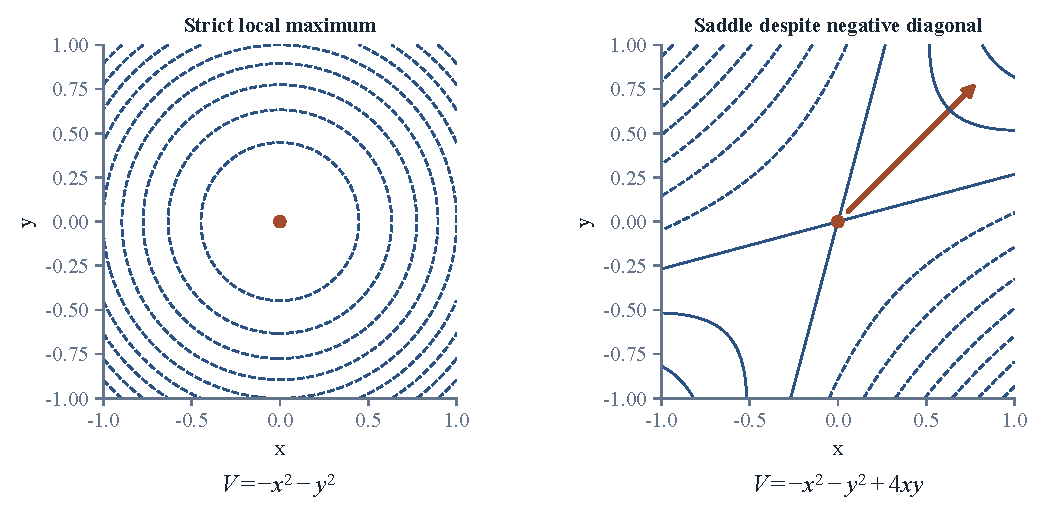
\includegraphics[width=\textwidth]{assets/hessian-directions.pdf}
\caption{Both Hessians have diagonal entries $-2$. The left Hessian is negative definite. The mixed term on the right creates eigenvalues of both signs, so the origin is a saddle and the red direction increases the score.}
\label{fig:mechanism-hessian-directions}
\end{figure}
If $V$ measures immediate satisfaction and retention, the system can reach a strong local position on those measures. Whether the position is good for users over time depends on what the objective includes and omits.

Nietzsche's “last man” supplies a literary image of satisfaction without aspiration \cite{nietzsche1883zarathustra}. The engineering account asks a different question: which valued dimensions can deteriorate without changing the score? Health, independent skill, reciprocal relationships, and public participation can all be weakly represented in a short feedback window.

Leaving a strict local maximum along a chosen path may require an initial score decline. Define the depth of that decline as
\begin{equation}
 \Delta V_{\mathrm{loss}}
 =V(x^\ast)-\min_{s\in\mathrm{path}}V(s)\geq0.
\end{equation}
The path includes the starting point. A larger value means a deeper temporary loss on that path. A universal escape barrier would additionally require optimization over admissible paths and a specified destination.

Who bears the interim loss? A service that reduces an engagement metric may lose revenue before a long-term benefit becomes measurable. A person practicing an old skill may produce less today while preserving a capability needed later. The immediate cost and delayed benefit appear on different schedules.

Changing the objective, adding constraints, creating competing services, or financing the transition can alter the path. Local optimality describes the geometry of the chosen score. Changing that score can change the way out.


\begin{figure}[ht]
\centering
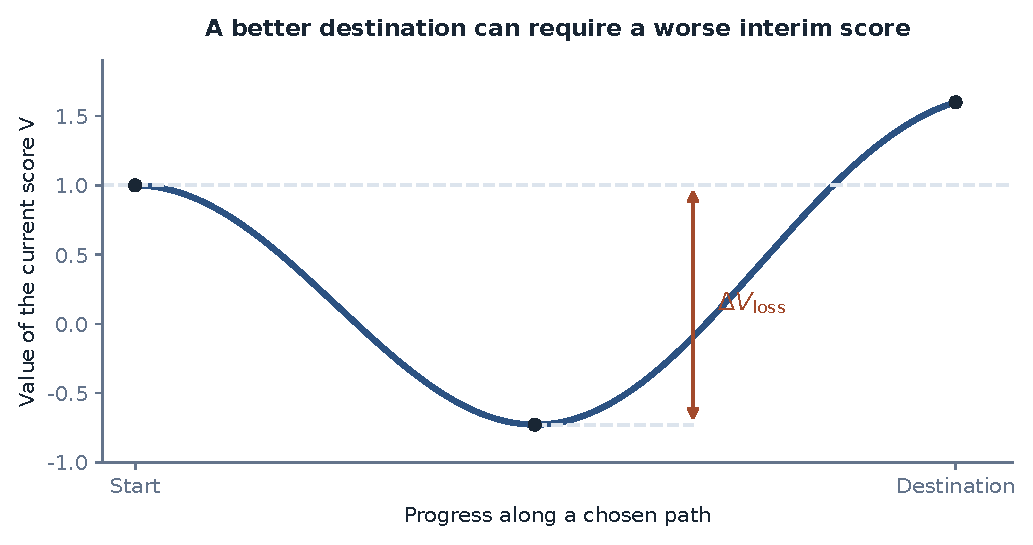
\includegraphics[width=\textwidth]{assets/escape-valley.pdf}
\caption{The temporary score loss on one chosen path is the starting value minus the minimum along that path. Including the start makes the loss nonnegative. A different objective, constraint, or feasible path can change it.}
\label{fig:mechanism-escape-valley}
\end{figure}
\subsection{Diversity as a Recovery Resource}

Many similar decisions can create a common exposure. Financial institutions using correlated models and funding structures can amplify a shock together \cite{haldane2011systemic}. Infrastructure needs alternatives that remain available after a failure; contingency standards are one way to preserve them \cite{morison2004power}.

Cultural and cognitive diversity are harder to measure but share one practical function: an alternative method can remain available when the dominant method fails. Preserving several routes consumes resources before the moment at which their value is obvious.

Recommendation systems can narrow or diversify exposure. User choices and network composition also matter. Research on cross-cutting information in Facebook showed that several mechanisms contributed, with effects that cannot be reduced to ranking alone \cite{bakshy2015exposure}. A claim about today's systems needs present measurements of today's design and use.

At the political level, Arendt's analysis emphasizes the danger of atomized people losing meaningful attachments in a common world \cite{arendt1951origins}. The useful implication is to preserve institutions in which people can participate, disagree, and obtain an answer. A platform's convenience cannot substitute for every such institution.

Automation can reduce the burden of judgment. It can also erode the practice needed for effective oversight when users become unable to evaluate a recommendation \cite{parasuraman1997humans}. The appropriate response supplies intelligible evidence, maintained skills, time, and real decision rights.

Agency survives through use and support. It needs occasions on which a person's reasons affect a process, relations in which commitments have reciprocal force, and institutions that keep objection possible. Convenience can support those conditions. Its quality should be judged by whether it does.
